\documentclass[a4paper]{article}

\usepackage{amsmath}
\usepackage{graphicx}
\usepackage{subcaption}
\usepackage{listings}
\usepackage{xcolor}
\usepackage{hyperref}
\usepackage[all]{hypcap}

\author{Xeryus Stokkel(s2332795)}
\title{Computer Vision lab 3: Inference}

\lstset{
	basicstyle=\footnotesize,
	breakatwhitespace=false,
	breaklines=true,
	frame=single,
	keepspaces=true,
	numbers=left,
	numbersep=5pt,
	numberstyle=\tiny,
	tabsize=4,
	rulecolor=\color{black},
	showspaces=false,
	showstringspaces=false,
	showtabs=false,
	title=\lstname,
	}

\begin{document}

\maketitle

\section*{Exercise 1}
Because we know that the opposite sides of a rectangle are parallel we can calculate the vanishing point of these two sides as follows. The equation that defines the projection of the sides is
\[ L = \left(\begin{array}{c}u\\v\end{array}\right) = \left\{ \left(\begin{array}{c} c_1\\c_2\end{array} \right) + \eta \left(\begin{array}{c} d_1\\d_2\end{array}\right) \right\} \]

When we have two lines we can find the vanishing point in the image plane by solving $L_1 = L_2$, this will give $u_\infty$ and $v_\infty$.

\section*{Exercise 2}
One set of parallel lines that has been scanned is shown in \autoref{fig:scanpoints}. The other set of parallel lines consists of the lines that are orthogonal to the red lines in \autoref{fig:scanpoints}.
\begin{figure}[h]
	\centering
	\begin{subfigure}[t]{.49\textwidth}
		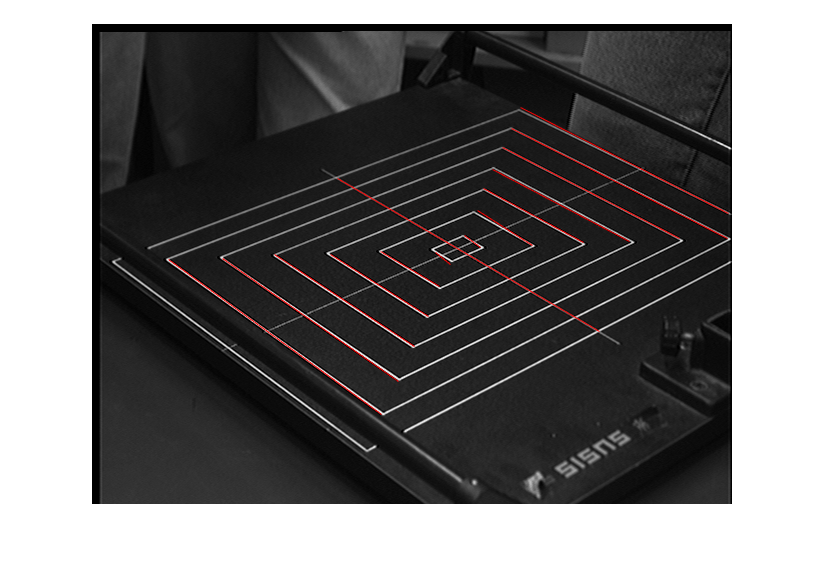
\includegraphics[width=\textwidth]{par_lines}
		\caption{The vertical set.}
	\end{subfigure}
	\begin{subfigure}[t]{.49\textwidth}
		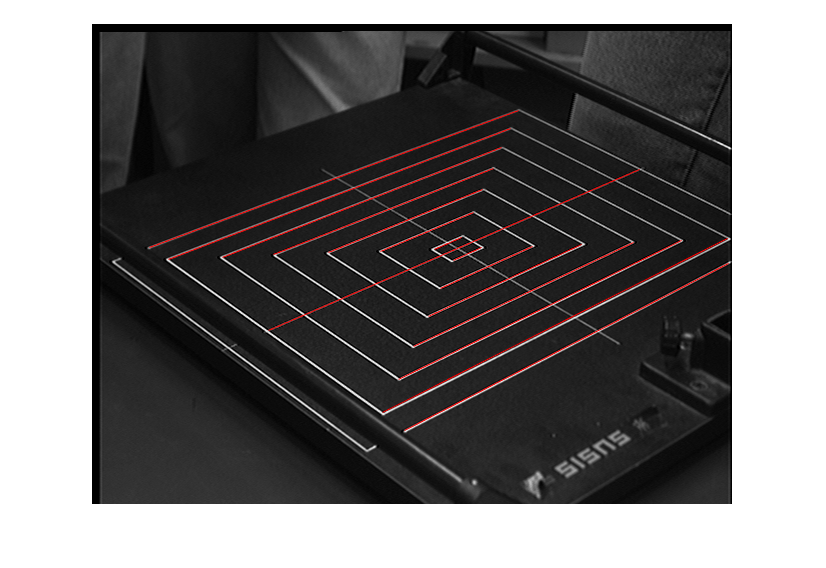
\includegraphics[width=\textwidth]{par_lines2}
		\caption{The horizontal set.}
	\end{subfigure}
	\caption{The two sets of parallel lines that have been scanned.}
	\label{fig:scanpoints}
\end{figure}

\section*{Exercise 3}
The files obtained from the sets in \autoref{fig:scanpoints} are shown below
\lstinputlisting[caption={The parallel lines for the vertical set}]{parlines1.dat}
\lstinputlisting[caption={The parallel lines for the horizontal set}]{parlines2.dat}

\section*{Exercise 4}

\end{document}